\chapter{Brownian Motion in Soft Confinement}

\section{Introduction}

In many biological systems, one must not only take into account Brownian behaviours, but also carefully evaluate the effect of the system's or parts of the system's deformability on its dynamics. Indeed, if we take the example of a lipid bilayer, which is a soft and quasi-two-dimensional fluid, the thermal energy $k_\mathrm{B}\Theta$ of the system is sufficient to cause long-wavelength bending fluctuations of the cell membrane, thickness fluctuations, lipid movement within the plane itself, and so forth. Naturally, a neighbouring fluid's motion is then affected by these shape modifications, which can in turn affect the dynamics of a body evolving in that same bath. This coupling is not trivial. I describe in this chapter what has already been developed on that matter, starting with the more well-established case of deterministic soft lubrication. I then present an overview of the stochastic case, where bodies or confinements are fluctuating and deformable. The remainder of the chapter is articulated around the presentation, development and numerical verifications of a simple and elementary model we developed during my doctoral contract to assess this same problematique of soft Brownian effects.

\subsection{Deterministic soft lubrication}




\subsection{Stochastic soft lubrication}
The aim of this chapter is to probe at these modifications to colloid's behaviour. 

Because of the level of complexity of such a study, I present in this chapter a most simple model, with elementary ingredients, which can still qualitatively capture all the effects we are interested in. Such model is detailed in the next section. In the following sections, I develop the numerical model used to simulate this toy model. I then present the theoretical aspects of the model, developed by David S. Dean. Finally, I show how numerics and theory compare.

\section{Toy Model for soft Brownian Motion}
\subsection{Overview of the Toy Model}

\begin{figure}
    \centering
    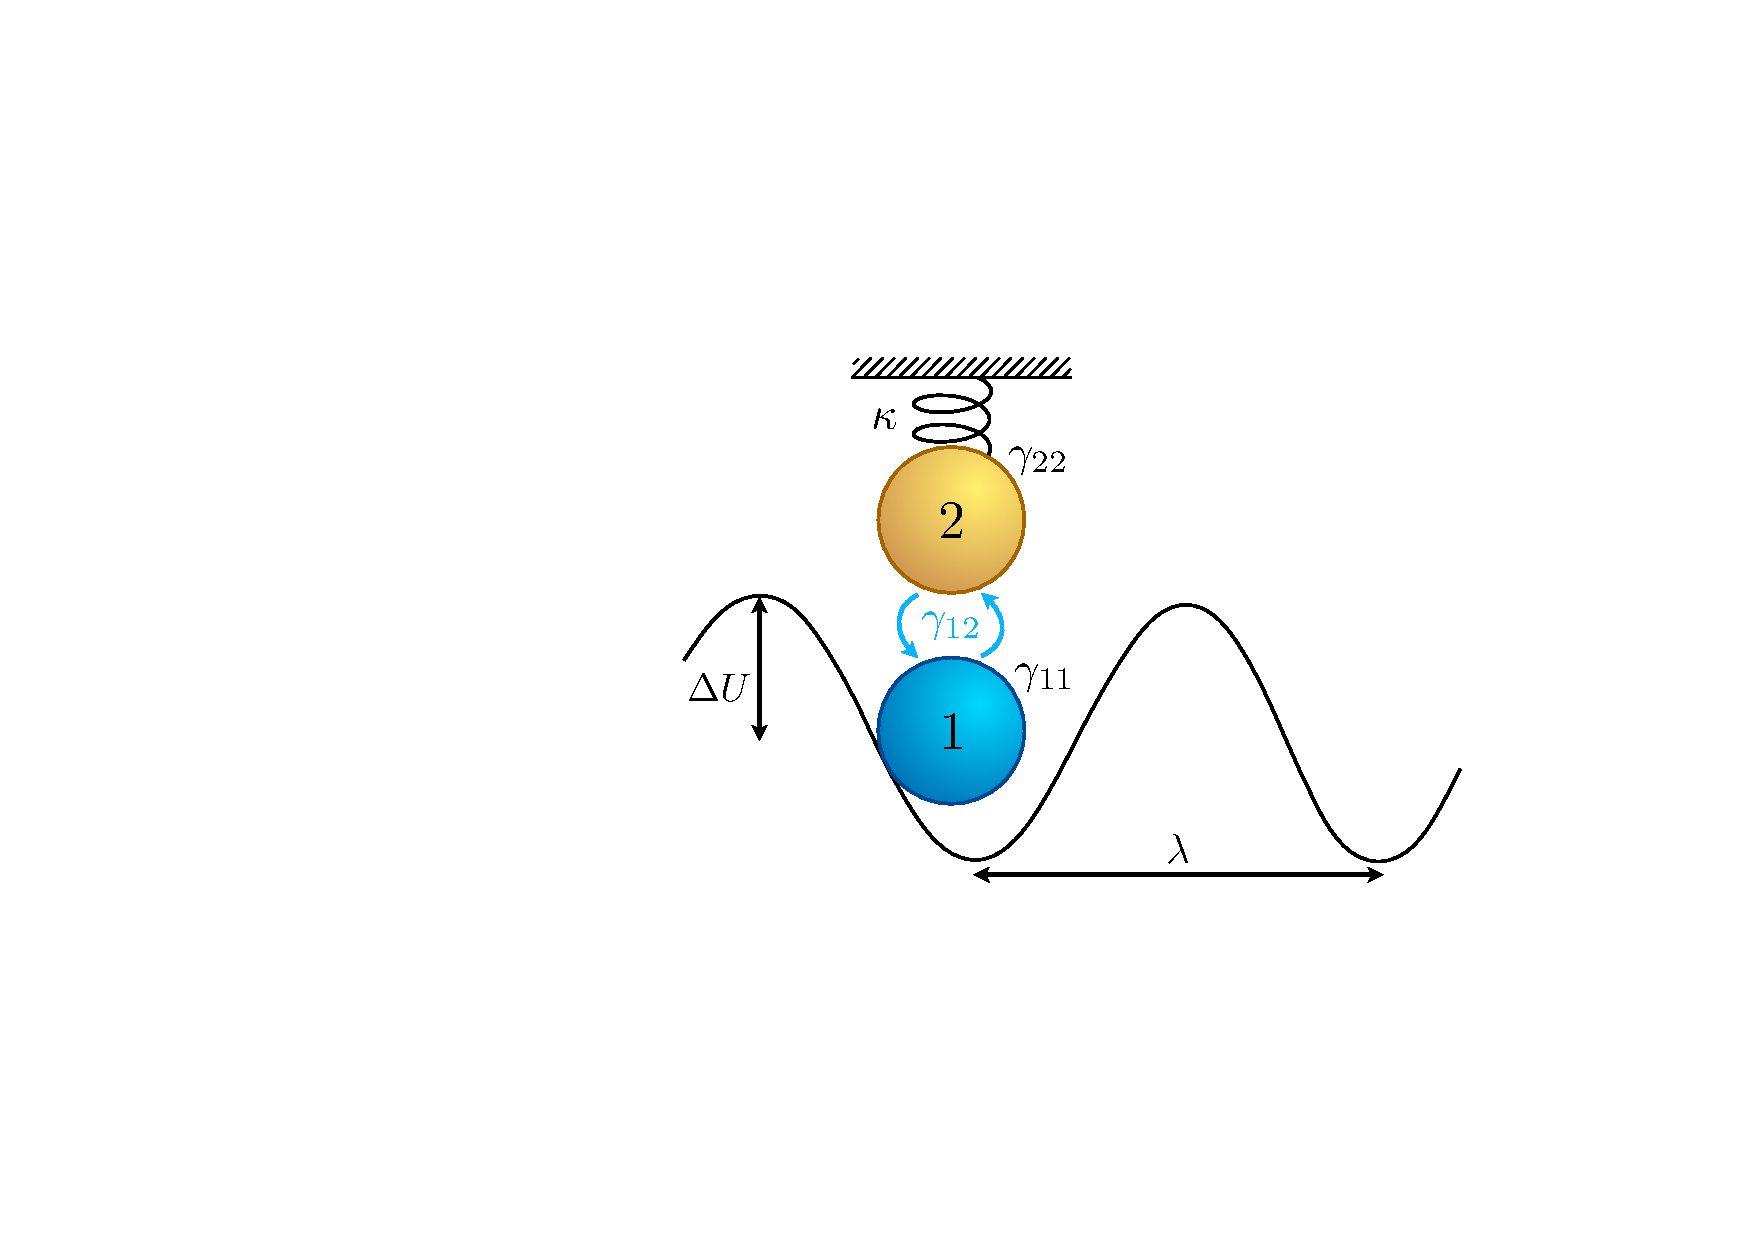
\includegraphics[width=0.8\textwidth]{figures/chapter3/toy_model_figure_1.pdf}
    \caption{Representation of the system. A Brownian colloid of interest (blue) is trapped in a periodic potential of amplitude $\Delta U$ and spatial period $\lambda$. An elastic membrane is modelled as a second Brownian colloid (orange) subject to a harmonic potential of inverse stiffness of compliance $\kappa$. This membrane is coupled to the colloid of interest through an indirect hydrodynamic coupling represented by the coefficient $\gamma_{12}$, and both the colloid and the membrane feel their own self-friction $\gamma_{11}$ and $\gamma_{22}$, respectively.}
    \label{toy_model_figure_1}

\end{figure}


From here on, we study a purely one-dimensional case of a Brownian colloid coupled to an elastic and fluctuating membrane (Fig. \ref{toy_model_figure_1}). The Brownian colloid is represented by a first degree of freedom, $q_1$, and is submitted to a periodic trapping potential $\phi(q_1)$ of spatial period $\lambda$ and amplitude $\Delta U$. Throughout this chapter, the Brownian colloid's degree of freedom $q-1$ will be color-coded in blue, and the membrane's degree of freedom $q_2$ in red. We couple to this colloid the toy model version of the membrane. We represent the membrane with a colloid that is submitted in a harmonic potential of energy $\frac{q_2^2}{2\kappa}$, where $\kappa$ is the compliance (or inverse stiffness). It represents the elasticity of the membrane. This second colloid is tracked with the second degree of freedom, $q_2$. 



Both the Brownian colloid and the membrane feel their own self-friction, respectively $\gamma_{11}$ and $\gamma_22$. Furthermore, they interact through and indirect, hydrodynamic-like interaction $\gamma_{12}$. This interaction represents the effect of the fluid that is displaced by the motion of the colloid on the membrane, and \emph{vice-versa}. All together, these terms form the friction matrix $\mathbf{\Gamma}$

\begin{equation}
    \mathbf{\Gamma} = \begin{pmatrix}
    \gamma_{11} & \gamma_{12} \\
    \gamma_{12} & \gamma_{22}
    \end{pmatrix}
\end{equation}

which can be inverted to give the mobility matrix of the system, as $\mathbf{M} = \mathbf{\Gamma}^{-1}$. Both matrices must be positive definite, and, because their diagonal terms account for the self-friction and self-mobility respectively, $\mu_{11} > 0$ and $\mu_{22} > 0$.   

We can write the total energy as

\begin{equation}
    H (q_1, q_2) = \phi(q_1) + \frac{q_2^2}{2\kappa}~,
\end{equation}

and we notice the absence of Hamiltonian interactions in the system. In that case, we work in the overdamped limit, and we write the coupled Langevin equations describing the evolutions of $q_1$ and $q_2$ as

\begin{align}
    \label{3ToyMod_langevin1}
    \gamma_{11}\frac{\mathrm{d}q_1}{\mathrm{d}t} + \gamma_{12}\frac{\mathrm{d}q_2}{\mathrm{d}t} &= -\phi'(q_1) + \eta_1(t)~, \\
    \gamma_{12}\frac{\mathrm{d}q_1}{\mathrm{d}t} + \gamma_{22}\frac{\mathrm{d}q_2}{\mathrm{d}t} &= -\frac{q_2}{\kappa} + \eta_2(t)~,
    \label{3ToyMod_langevin2}
\end{align}

where $\eta_i$ and $\eta_j$ (with $j \in \{1, 2\}$) are Gaussian white noises of zero mean and correlation functions $\langle \eta_i(t) \eta_j(t')\rangle = 2 k_\mathrm{B}T \delta(t - t')\gamma_{ij}$.


\begin{equation}
    P_\mathrm{eq} = \frac{\exp[-\beta H(q_1, q_2)]}{Z}~,
    \label{P_eq}
\end{equation}



%%%%%%%%%%%%%%%%%%%%%%%%%%%%%%%%%%%%%%%%%%%%%%%%%%%%%%%%%%%%%%%%%%%%%%%%%%%%%%%%%%%%%%%%%%%%%%%%%%%%%%%%%%%%%%%%%%%%%%%%%%%%%%%%%%%%%%%
\section{Theoretical developments}

The objective of the following developments is to compute the modification to the long-time dynamics of the Brownian colloid diffusing within the sinusoidal trap. The development I choose to present here is not the most rigorous, and corresponds to the very stiff ($\kappa \to 0$) limit of the elastic membrane. The interested reader can find a more rigorous argument in the appendices of this thesis, alongside a second development for the very compliant limit ($\kappa \to \infty$). 


We begin by refactoring Eqs. \ref{3ToyMod_langevin1} and \ref{3ToyMod_langevin2} in the deterministic case $\Theta = 0$ 


\begin{align}
    \label{3ToyMod_athermal_q1}
    \frac{\mathrm{d}q_1}{\mathrm{d}t} & = -\mu_{11} \phi'(q_1) - \frac{\mu_{12}}{\kappa}q_2~, \\
    \frac{\mathrm{d}q_2}{\mathrm{d}t} & = -\mu_{12} \phi'(q_1) - \frac{\mu_{22}}{\kappa}q_2~. 
\end{align}

We may then integrate to express $q_2$ as

\begin{equation}
    q_2 = - \frac{\kappa \mu_{12}}{\mu_{22}} \left( 1 + \frac{\kappa}{\mu_22} \frac{\mathrm{d}}{\mathrm{d}t}\right)^{-1} \phi'(q_1)~.
\end{equation}


In the small $\kappa$ limit, we then expand the right-hand bracket term, taking into account the chain rule
\begin{equation}
    q_2 \simeq - \frac{\kappa \mu_{12}}{\mu_{22}} \left[ \phi'(q_1) - \frac{\kappa}{\mu_{22}}\phi''(q_1) \frac{\mathrm{d}q_1}{\mathrm{d}t} + O(\tau_2^2)\right]~.
\end{equation}

Here, we note that $\tau_2$ is the characteristic relaxation time of the harmonic trapping corresponding to the membrane elasticity, as $\tau_2 = \frac{\kappa}{\mu_{22}}$. Now, substituting this new expression for $q_2$ in Eq. \ref{3ToyMod_athermal_q1}, we obtain

\begin{equation}
     \frac{\mathrm{d}q_1}{\mathrm{d}t} = - \left( \mu_{11} - \frac{\mu_{12}^2}{\mu_{22}}\right) \phi'(q_1(t)) - \frac{\kappa \mu_{12}^2}{\mu_{22}^2} \phi''(q1(t)) \frac{\mathrm{d}q_1}{\mathrm{d}t}~,
\end{equation}

which we can reexpress as

\begin{equation}
    \frac{\mathrm{d}q_1}{\mathrm{d}t} = -\mu_\mathrm{e}(q_1)\phi'(q_1)~,
    \label{3ToyMod_q1mue}
\end{equation}

where $\mu_\mathrm{e}$ is a dressed mobility with expression

\begin{equation}
    \mu_\mathrm{e} = \frac{\mu_{11}\mu_{22} - \mu_{12}^2}{\mu_{22}\left( 1 + \frac{ \kappa \phi''(q_1) \mu_{12}^2}{\mu_{22}^2}\right)}~.
\end{equation}

Remembering that $\mathbf{\Gamma} = \mathbf{M}^{-1}$, 

\begin{equation}
    \mu_\mathrm{e} = \frac{1}{\gamma_{11}\left( 1 + \frac{ \kappa \phi''(q_1) \mu_{12}^2}{\mu_{11}^2}\right)}~.
\end{equation}


Now, we can avoid reexpressing the noise should be added to Eq. \ref{3ToyMod_q1mue} for the thermal case by working directly with Fokker-Planck formalism. This formalism is introduced in its elementary form at the beginning of my thesis, and developed for more complex cases in Chapter 2. \textcolor{red}{CHECK CHAPT NR AT THE END OF THE REDACTION HERE} Doing such a thing is not rigorous, as I previously mentioned, because the effective stochastic process has not been derived. Eliminating fast variables in Eq. \ref{3ToyMod_q1mue} typically introduces non-trivial corrections. However, since we assume separation of timescales, the effective slow process still permits the writing of a uniquely-defined Fokker-Plank equation. 

This Fokker-Plank equation reads

\begin{equation}
    \frac{\partial P_1 (q_1, t)}{\partial t} = \frac{\partial}{\partial q_1} \mu_\mathrm{e}(q_1) \left[ k_\mathrm{B}\Theta \frac{\partial P_1 (q_1, t)}{\partial q_1} + \phi'(q_1)P_1(q_1, t)\right]
\end{equation}


and, noting that the time derivative of the probability density function $P_1(q_1, t)$ can be expressed in terms of probability flux $J(q_1, t)$,


\begin{equation}
    \frac{\partial P_1(q_1, t)}{\partial t} = -\frac{\partial J}{\partial q_1~.}
\end{equation}

This allows us to write

\begin{equation}
    J(q_1, t) = -D_\mathrm{e}(q_1) \frac{\partial}{\partial q_1} P_1(q_1, t) - \mu_\mathrm{e} \phi'(q_1) P_1(q_1, t)~,
\end{equation}


where $D_\mathrm{e} = k_\mathrm{B}\Theta$. The above equation can be rewritten 

\begin{equation}
    J = - D_\mathrm{e}(q_1)\exp\left[-\beta \phi(q_1)\right] \frac{\mathrm{d}}{\mathrm{d}q} \left\{\exp\left[\beta \phi(q_1)\right]P_1 (q_1, t)\right\}
\end{equation}

with $\beta = \frac{1}{k_\mathrm{B}\Theta}$.

Now, we tilt the potential by adding a small force $F$, which gives a new potential $U(q_1)$

\begin{equation}
    U(q_1) = \phi(q_1) - Fq_1~.
\end{equation}

Then, the current equation can be rewritten taking account this new force, and gives

\begin{equation}
    \frac{\mathrm{d}}{\mathrm{d}q_1} \left\{ \exp[\beta U(q_1)] P(q_1, t)\right\} = - \frac{J(q_1, t)}{D_\mathrm{e}(q_1)} \exp[\beta U(q_1)]~.
\end{equation}

We can then integrate over a period $\lambda$, and, using periodicity, we retrieve

\begin{equation}
    P_1(q_1, t) = \frac{J(q_1) \exp[-\beta U(q_1)]}{1 - \exp(-\beta F \lambda)} \int_{q_1}^{q_1 + \lambda} \frac{\exp[\beta U(q)]}{D_\mathrm{e}(q)}\mathrm{d}q~.
\end{equation}

\textcolor{red}{check J(q, t) or just q.}

By essence, $P_1(q_1, t)$ is normalised

\begin{equation}
    \int_{0}^{\lambda}P_1(q_1)\mathrm{d}q_1 = 1~,
\end{equation}

and thus we retrieve for $J$

\begin{equation}
    J(q_1) = \frac{1 - \exp[-\beta F \lambda]}{\int_{0}^{\lambda} \exp[-\beta U(q)]\mathrm{d}q \int_{q}^{q+\lambda} \frac{\exp[\beta U(q)]}{D_\mathrm{e}(q)}\mathrm{d}q}~.
\end{equation}


In the small force limit $F \to 0$,

\begin{equation}
    1 - \exp(-\beta F \lambda)  \simeq \beta F \lambda~,
\end{equation}

which, to leading order in $F$, gives

\begin{equation}
    J(q_1) = \frac{\beta F \lambda}{\int_{0}^{\lambda} \exp[-\beta \phi(q_1)] \mathrm{d}q_1 \int_{0}^{\lambda} \frac{\exp[\beta \phi(q_1)]}{D_\mathrm{e}(q_1)}\mathrm{d}q_1}~.
\end{equation}

Finally, we note that the drift velocity should read $v = J(q_1) \lambda$, and that the effective diffusion coefficient over $\lambda$ should be 

\begin{equation}
    D^* = \frac{k_\mathrm{B}\Theta v}{F} = \frac{\lambda^2}{\int_{0}^{\lambda} \exp[-\beta \phi(q_1)]\mathrm{d}q_1 \int_{0}^{\lambda} \frac{\exp(\beta \phi(q_1))}{D_\mathrm{e}(q_1)}\mathrm{d}q_1}~,
\end{equation}

which is the generalised Lifson-Jackson formula. \textcolor{red}{cite.}


Finally, we replace $D_\mathrm{e}(q_1)$ in the expression 


\begin{equation}
    D^* = \frac{k_\mathrm{B}\Theta\lambda^2}{\gamma_{11}\int_{0}^{\lambda} \mathrm{d}q \exp[\beta \phi(q)] \left(1 - \frac{\kappa \gamma_{12}^2 \phi'^2(q)}{k_\mathrm{B}\Theta \gamma_{11}^2}\right) \int_{0}^{\lambda} \mathrm{d}q \exp[-\beta \phi(q)]}
\end{equation}


And, by expansion in very small $\kappa$, and setting $\phi(q_1) = \Delta U \phi(\frac{q_1}{\lambda})$, where $\Delta U$ is the amplitude of the periodic trap

\begin{equation}
    D^* = \frac{k_\mathrm{B}\Theta}{\gamma_{11}\int_{0}^{1} \mathrm{d}p \exp[\beta\Delta U \psi(p)] \left(1 - \frac{\kappa \gamma_{12}^2 \Delta U^2\psi'^2(p)}{k_\mathrm{B}\Theta \gamma_{11}^2}\right) \int_{0}^{1} \mathrm{d}p \exp[-\beta \Delta U\psi(p)]}~.
    \label{D_star}
\end{equation}

\textcolor{blue}{here.}



%%%%%%%%%%%%%%%%%%%%%%%%%%%%%%%%%%%%%%%%%%%%%%%%%%%%%%%%%%%%%%%%%%%%%%%%%%%%%%%%%%%%%%%%%%%%%%%%%%%%%%%%%%%%%%%%%%%%%%%%%%%%%%%%%%%%%%%
\section{Numerical modelling}
\subsection{Discretisation}
My main mission in this project is to simulate the above Eqs. \ref{3ToyMod_langevin1} and  \ref{3ToyMod_langevin2} efficiently. To do so, I discretise these equations using a simple forward Euler scheme (which was introduced in the beginning of this thesis). The equations read

\begin{align}
    \label{q1_discretized}
    q_1(t + \Delta t) - q_1(t) &= -\mu_{11} \phi'(q_1(t))\Delta t - \frac{\mu_{12}}{\kappa}q_2(t)\Delta t + \xi_1 \sqrt{2k_\mathrm{B}T\Delta t}~,\\
q_2(t + \Delta t) - q_2(t) &=  - \frac{\mu_{22}}{\kappa}q_2(t)\Delta t -\mu_{12} \phi'(q_1(t))\Delta t + \xi_2 \sqrt{2k_\mathrm{B}T\Delta t}~, \label{q2_discretized}
\end{align}

where $\xi_i$ is a zero-mean Gaussian random variable, as

\begin{equation}
    \langle \xi_i \xi_j \rangle = \mu_{ij}~.
\end{equation}

We choose to work in terms of mobility instead of friction matrix elements for convenience in the upcoming developments. They are, however, strictly equivalent.

Furthermore, in the rest of this study, we choose $\phi(q_1)$ to be sinusoidal, as $\phi(q_1) = \Delta U \sin\left(\frac{2 \pi q_1}{\lambda}\right)$,
with $\Delta U$ the amplitude of the sinusoidal trap. 

\subsection{Time step selection}

In any discretisation process, it is essential to choose the appropriate time step. This time step must be small enough to avoid a blowup from error propagation (again, see the beginning of this thesis for more details on how the Euler method propagates errors), but big enough to remain advantageous. An arbitrarily small timestep may prohibit the probing of very long time dynamics due to computation time. 

To select a correct time step for a simulation, I typically first identify all the smaller time scales in the system I want to simulate. In the present study, I identify two time scales : the local relaxation time within a local minimum of the sinusoidal trap, and the relaxation time of the harmonic trap. 

Near a local minimum, we may approximate the sinusoidal trap as harmonic. In that case, 

\begin{equation}
    \phi(q_1) = \frac{1}{2} k_\mathrm{eff}q_1^2~,
\end{equation}

where $k_\mathrm{eff}$ is an effective stiffness, which we identify as the local curvature of the potential as 

\begin{align}
k_\mathrm{eff} &= |\phi''(0)| \\
&= \Delta U \left( \frac{2 \pi}{\lambda} \right)^2~,
\end{align}

and we can finally identify this first timescale as

\begin{equation}
    \tau_1 = (\mu_{11} k_\mathrm{eff})^{-1} = \frac{\lambda^2}{4 \pi^2 \Delta U \mu_{11}}~.
\end{equation}

The harmonic trap is much simpler, as it requires no approximations, and we find its characteristic timescale 

\begin{equation}
    \tau_2 = \frac{\kappa}{\mu_{22}}~.
\end{equation}

Then, I choose a time step which satisfies

\begin{equation}
    \Delta t = \frac{1}{100}\max{\tau_1, \tau_2}~.
\end{equation}


We also need to define an upper bound to the simulation time. We must always remain mindful of the computational cost of our simulations, as time and energy both are scarce resources. Thus, we can define a time scale $\tau^*$ which depends on the long-time effective diffusion coefficient $D^*(\kappa)$ defined in Eq. \ref{D_star}

\begin{equation}
    \tau^*(\kappa) = \frac{\lambda^2}{D^*(\kappa)}~.
\end{equation}


I choose to run my simulations for a time $T_\mathrm{sim}$ which is much larger than $\tau^*$, as $T_\mathrm{sim} = 100 \tau^*$. This allows me to probe the long-time dynamics of the system, and to extract the effective diffusion coefficient from the mean-squared displacement of the Brownian colloid. This, in turn, sets the computational cost of a simulation, which I can quantify using the total number of iterations in the time loop $N$ as

\begin{equation}
    N = \frac{T_\mathrm{sim}}{\Delta t} = \frac{100 \tau^*}{\Delta t}~ .
\end{equation}





%%%%%%%%%%%%%%%%%%%%%%%%%%%%%%%%%%%%%%%%%%%%%%%%%%%%%%%%%%%%%%%%%%%%%%%%%%%%%%%%%%%%%%%%%%%%%%%%%%%%%%%%%%%%%%%%%%%%%%%%%%%%%%%%%%%%%%%
\section{Results}

The interested reader can find a minimal version of a trajectory generation code \textcolor{red}{here}. This simple code allows the user to tune parameters and test for themself their effect on the dynamics of the system. I also provide all data treatment codes for archiving purposes, and will be referring to parts of it in this manuscript. Most of the figures presented in this section are generated using this simpler script, in which I left the seed fixed to ensure proper reproducibility.

\subsection{Trajectories}

I first generate trajectories of the two coupled Brownian colloids using Eqs. \ref{3ToyMod_athermal_q1} and \ref{3ToyMod_athermal_q2}, for a given set of parameters. A sample of a single trajectory is shown in Fig. \ref{Trajectories}. We can see that the membrane fluctuates around its equilibrium position in $q_2 = 0$, whereas the Brownian colloid is trapped at short times within a local minimum, and escapes through random thermal fluctuations at longer times to explore space. This is a first verification that the simulations are workign as expected. Indeed, it is not unusual for Brownian simulations to blowup in the case of an unfortuitous dimensionalisation of the system, and this issue is almost always imputable to a too-large time step. We have already discussed this matter in the beginning of the manuscript. 


\begin{figure}
    \centering
    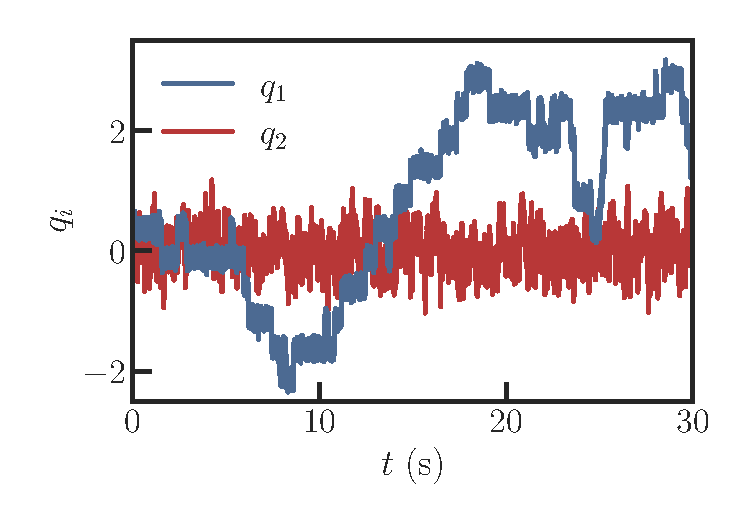
\includegraphics[width=0.8\textwidth]{figures/chapter3/Trajectories.pdf}
    \caption{Trajectories of the Brownian colloid (blue) and the membrane (red) for $\kappa = 0.01$. The other parameters are fixed to $\Delta U = 1.0 k_\mathrm{B}\Theta$, $\lambda = 1.0$, $\gamma_{11} = 1$, $\gamma_{22} = 1$ and $\gamma_{12} = 0.8$, $\tau = 10^{-4}$. The membrane noticeably fluctuates around its equilibrium position in $q_2 = 0$, whereas the colloid is trapped at short times within a local minimum, and escapes through random thermal fluctuations at longer times to explore space. }
    \label{Trajectories}
\end{figure}

We may verify the behaviour of the system at equilibrium by sampling the probability density function of $q_1$ and $q_2$ from the generated trajectories, and comparing them to the theoretical prediction from the Gibbs-Boltzmann distribution (Eq. \ref{P_eq}). This is shown in Figs. \ref{Peq_q1} and \ref{Peq_q2}. We can see that the sampled probability density functions (histograms) and theoretical prediction from the Gibbs-Boltzmann distribution (solid lines) are in perfect agreement, even for weak statistics. The sampled probability distribution of $q_1$ follows the expected periodic shape, whereas the one of $q_2$ follows the expected Gaussian shape predicted by Eq. \ref{P_eq}. This is a second verification that the simulations are working as expected, and that we are correctly sampling the equilibrium distribution of the system.



\begin{figure}
    \centering
    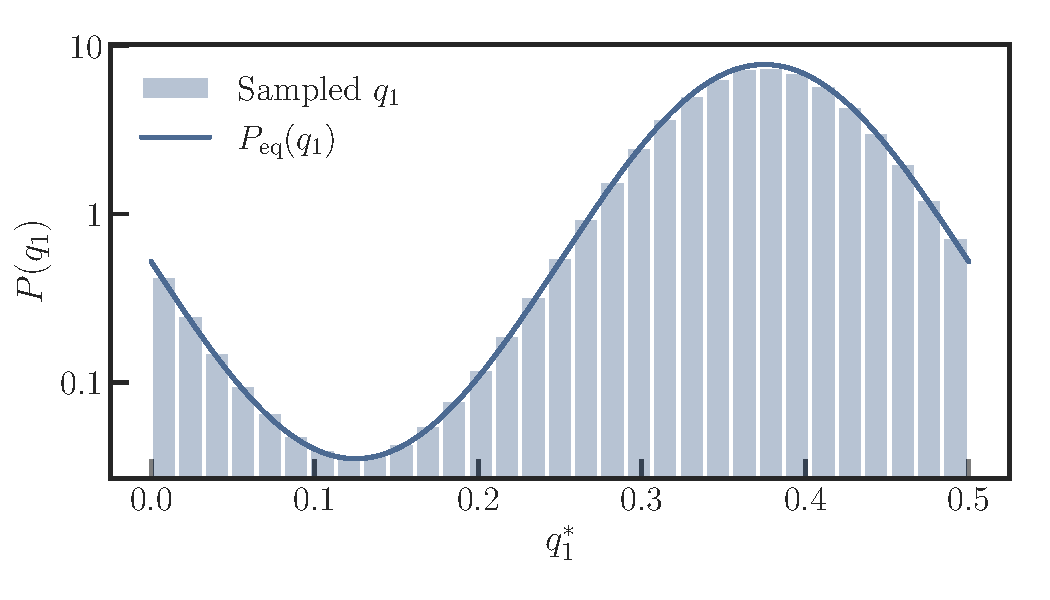
\includegraphics[width=0.8\textwidth]{figures/chapter3/Peq_q1.pdf}
    \caption{Equilibrium probability density function of $q_1$ for $\kappa = 0.01$. The other parameters are fixed to $\Delta U = 1.0 k_\mathrm{B}\Theta$, $\lambda = 1.0$, $\gamma_{11} = 1$, $\gamma_{22} = 1$, $\gamma_{12} = 0.8$, $\tau = 10^{-4}$, for a single trajectory of $N=1\times 10^7$ points. The sampled probability density functions (histograms) and theoretical prediction from the Gibbs-Boltzmann distribution (Eq. \ref{P_eq}, solid lines) are in perfect agreement, even for weak statistics.}
    \label{Peq_q1}
\end{figure}

\begin{figure}
    \centering
    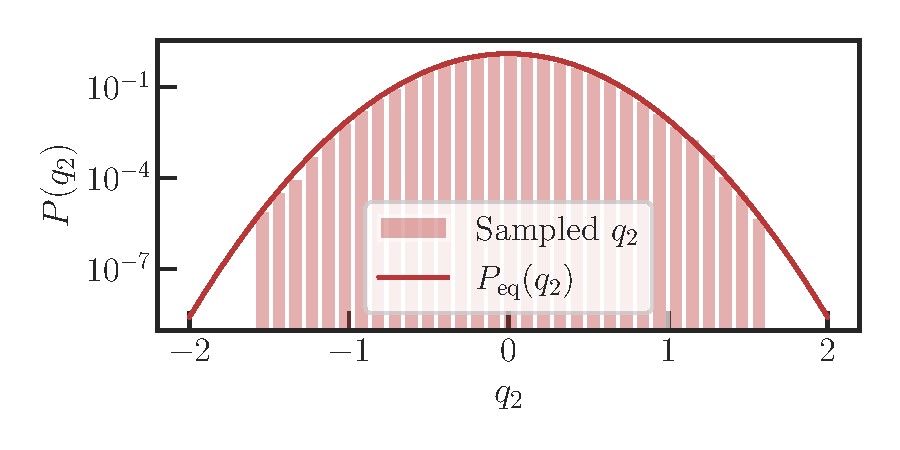
\includegraphics[width=0.8\textwidth]{figures/chapter3/Peq_q2.pdf}
    \caption{Equilibrium probability density function of $q_2$ for $\kappa = 0.01$, $\Delta U = 1.0 k_\mathrm{B}\Theta$, $\lambda = 1.0$, $\gamma_{11} = 1$, $\gamma_{22} = 1$, $\gamma_{12} = 0.8$, $\tau = 10^{-4}$, for a single trajectory of $N=1\times 10^7$ points. Again, the sampled probability distribution (histograms) follows the expected Gaussian shape predicted by Eq. \ref{P_eq} (solid lines).}
    \label{Peq_q2}
\end{figure}


However, at this stage, we have not probed the dynamics of the system. Thus, we still have no insight on the effect of a sfot membrane on the diffusion of the Brownian colloid. To do so, we will need to compute the MSD of $q_1$ and $q_2$ from the generated trajectories, and to extract the effective diffusion coefficient of $q_1$ from the long-time behaviour of its MSD. We will then be able to compare this effective diffusion coefficient to the theoretical prediction from Eq. \ref{D_star}.


\subsection{Mean-Squared displacements}
For simplicity, I chose to compute the MSD of $q_1$ and $q_2$ using the standard definition of the MSD, as we defined it in the beginning of the manuscript. In that cse, the MSD is computed directly from the generated trajectories, calculating the average of the squared displacements over all possible or given time lags.

This technique is sufficient for the current study and for demonstration purposes. However, in our published work and in similar numerical studies \cite{millan_numerical_2023}, it is more convenient to first compute the histograms of \emph{displacements} at given time lags. This histogram can then be used to compute the MSD alongside other statistical moments of interest, such as the skewness and kurtosis. It also has the advantage of being a stackable quantity, which means that on a rolling basis as multiple trajectories are calculated, we may simply add counts to the historgam of displacements. 

This technique has a secondary convenient effect of giving a simple criterion on the stability of the results. We can define a convergence criterion on the histogram of displacements as the relative distance between a "previous" histogram of cumulative displacements, and an "updated" histogram which contains all previous iteration plus the new additions from the lastest simulated trajectories. When this relative distance is smaller than a given threshold for a sufficient number of iterations, we deem the simulation to have converged, and it automatically stops. This is a convenient way of saving resources and active working time, as it allows full automatisation of the whole process.

I define the convergence criterion as

\begin{equation}
    \epsilon = \frac{\sum_i |P_i^\mathrm{prev} - P_i^\mathrm{updated}|}{\sum_i P_i^\mathrm{prev}}~,
\end{equation}

where $P$ is the histogram of displacements, and $i$ the index of the bin. I choose a threshold of $\epsilon \leq 5\times10^{-3}$ for more than 3 iterations of 10 stacked trajectory statistics. This means that, when the relative distance between the "previous" and "updated" histograms of displacements is smaller than $5\times10^{-3}$ for more than 3 iterations of 10 stacked trajectories, we consider the simulation to have converged, and it automatically stops.

The results of a typical MSD calculation for $q_1$ and $q_2$ are shown in Figs. \ref{MSD_q1} and \ref{MSD_q2}. We can see that the MSD of $q_1$ (Fig. \ref{MSD_q1}) is at first diffusive with a $\Delta t$ exponent of 1 and a diffusion coefficient $D_\mathrm{m}$ whch is directly proportional to the self-mobility of the Brownian colloid as $D_\mathrm{m} = k_\mathrm{B}\Theta \mu_{11}$. It then falls into a slow crossover to reach a second diffusive regime of effective diffusivity $D^*$ as defined in Eq. \ref{D_star}. The long-time diffusion coefficient is smaller than the short-time diffusion coefficient, which is a signature of the trapping effect of the sinusoidal potential. 

\textcolor{blue}{add here : no coupling case.}


\begin{figure}
    \centering
    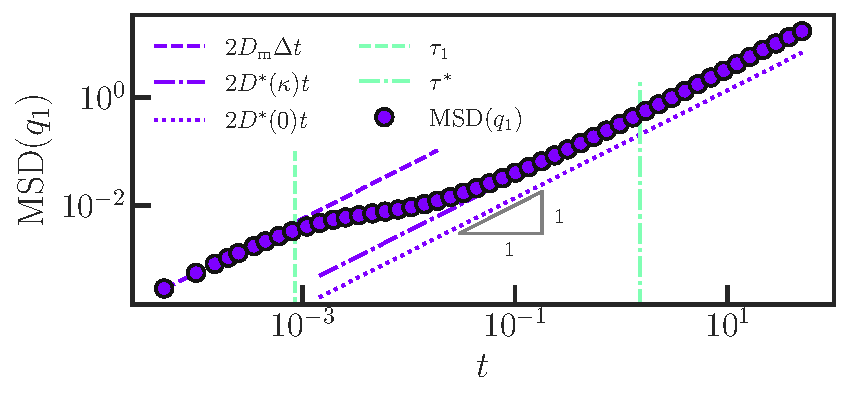
\includegraphics[width=0.8\textwidth]{figures/chapter3/MSD_q1.pdf}
    \caption{Mean-Squared Displacement of $q_1$ for $\kappa = 0.01$, $\Delta U = 1.0 k_\mathrm{B}\Theta$, $\lambda = 1.0$, $\gamma_{11} = 1$, $\gamma_{22} = 1$, $\gamma_{12} = 0.8$, $\tau = 10^{-4}$, for a single trajectory of $N=1\times 10^7$ points.}
    \label{MSD_q1}
\end{figure}

\begin{figure}
    \centering
    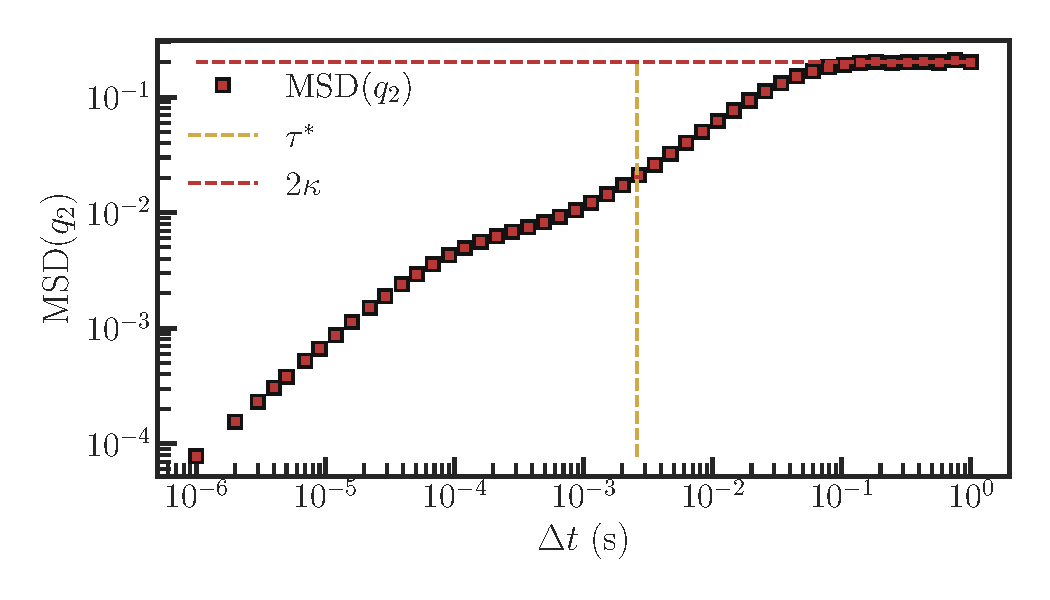
\includegraphics[width=0.8\textwidth]{figures/chapter3/MSD_q2.pdf}
    \caption{Mean-Squared Displacement of $q_2$ for $\kappa = 0.01$, $\Delta U = 1.0 k_\mathrm{B}\Theta$, $\lambda = 1.0$, $\gamma_{11} = 1$, $\gamma_{22} = 1$, $\gamma_{12} = 0.8$, $\tau = 10^{-4}$, for a single trajectory of $N=1\times 10^7$ points.}
    \label{MSD_q2}
\end{figure}

\subsection{Quantification of diffusion enhancement}


%%%%%%%%%%%%%%%%%%%%%%%%%%%%%%%%%%%%%%%%%%%%%%%%%%%%%%%%%%%%%%%%%%%%%%%%%%%%%%%%%%%%%%%%%%%%%%%%%%%%%%%%%%%%%%%%%%%%%%%%%%%%%%%%%%%%%%%
\section{Conclusion and perspectives on the chapter}